%Dạng 1
\section{Phương trình cân bằng nhiệt}
\subsection{Kiến thức cần nhớ}
\begin{khung}
	\subsubsection{Phương trình cân bằng nhiệt dạng cơ bản}
	\begin{itemize}
		\item Nhiệt lượng: $Q = mc\Delta t$\\ 
		Trong đó: $m$ là khối lượng; $c$ là nhiệt dung riêng; $\Delta t$ là độ biến thiên nhiệt độ. Đại lượng $C = mc$ được gọi là \textit{nhiệt dung}.
		\item Giả sử vật $m_{1}$ có nhiệt độ $t_{1}$ thả vào vật $m_{2}$ đang có nhiệt độ $t_{2}$ (giả sử $t_{1} > t_{2}$) $\to$ xảy ra sự trao đổi nhiệt, vật $m_{1}$ sẽ tỏa nhiệt, vật $m_{2}$ sẽ thu nhiệt đến khi nhiệt độ của hệ $(m_{1} + m_{2})$ đạt đến nhiệt độ cân bằng.
		
	\end{itemize}
	\subsubsection{Sử dụng phương pháp năng lượng} 
	Khi khó xác định được chất nào tỏa nhiệt (thu nhiệt) hay có nhiều chất cùng tham gia trao đổi nhiệt, ta sử dụng phương pháp bảo toàn năng lượng. Ta thấy, trong một hệ kín về nhiệt, sự thay đổi nhiệt năng của hệ bằng $0$, tức là tổng đại số nhiệt lượng các vật thu vào và tỏa ra bằng $0$.
	\hspace{1pt}
	\begin{center}
		$Q_{1} + Q_{2} + Q_{3} + \ldots = 0$
	\end{center}
	
\end{khung}
\subsection{Bài tập mẫu}
\Opensolutionfile{ans}[ans/ANS-DANG-1]
\begin{vd}%[Nguyễn Tấn Linh]%[2H2B1-1]
	[Đề minh họa BDG 2019-1020] 
	Từ một nhóm học sinh $6$ nam và $8$ nữ. Có bao nhiêu cách chọn ra một học sinh?
	\choice
	{\True $14$}	
	{$48$}
	{$6$}
	{$8$}
	\loigiai{
	\begin{phantich}
		\muccon{Dạng toán:}
			Đây là dạng toán quy tắc đếm, cụ thể là quy tắc cộng.\\
		\muccon{Hướng giải:}
			\begin{enumerate}[\bf B1.]
				\item Số cách chọn $1$ học sinh nữ từ $8$ học sinh nữ có $8$ cách.
				\item Số cách chọn $1$ học sinh nam từ $6$ học sinh nam có $6$ cách. 
				\item Số cách chọn ra một học sinh là $8+6=14$.
			\end{enumerate}
			Từ đó, ta có thể giải bài toán cụ thể như sau:
	\end{phantich}
	\textit{Cách 1.} Số cách chọn $1$ học sinh nữ từ $8$ học sinh nữ có $8$ cách.\\
	Số cách chọn $1$ học sinh nam từ $6$ học sinh nam có $6$ cách Số cách chọn ra một học sinh là $8+6=14$.\\
	\textit{Cách 2.} Tổng số học sinh là $8+6=14$.\\
	Số cách chọn $1$ học sinh nữ từ $14$ học sinh có $14$ cách.
	}
\end{vd}
\subsection{Bài tập tương tự và phát triển}
%%==========Câu 1
%%==========Câu 2
%%==========Câu 3
%%==========Câu 4
%%==========Câu 5
%%==========Câu 6
\begin{ex}%[Nguyễn Tấn Linh]%[1D2Y1-2]
%%==========Câu 7
\begin{ex}%[Nguyễn Tấn Linh]%[1D2Y1-3]
	Từ thành phố A có 10 con đường đi đến thành phố B, từ thành phố A có 9 con đường đi đến thành phố C, từ thành phố B đến thành phố D có 6 con đường, từ thành phố C đến thành phố D có 11 con đường và không có con đường nào nối B với C. Hỏi có bao nhiêu cách đi từ thành phố A đến thành phố D?
	\choice
	{$156$}
	{\True $159$}
	{$162$}
	{$176$}
	\loigiai{
		\begin{center}
			\begin{tikzpicture}[>=stealth,line join=round,line cap=round,font=\footnotesize,scale=1]
			\coordinate[label=above left:$A$](A) at (0,0);
			\coordinate[label=above:$B$](B) at (3,0); 
			\coordinate[label=below :$C$](C) at (2,-2);
			\coordinate[label=right:$D$](D) at (5,-1);
			\draw[line width=0.7pt,black] (A)--(B)node[above,pos=0.5]{10 con đường}; 
			\draw[line width=0.7pt,black] (B)--(D)node[above right,pos=0.5]{6 con đường};
			\draw[line width=0.7pt,black] (A)--(C)node[right,pos=0.5]{9 con đường};
			\draw[line width=0.7pt,black] (C)--(D)node[below right,pos=0.5]{11 con đường};
			\end{tikzpicture}
		\end{center}
		Phương án 1: đi từ A đến B rồi đến D.\\
		Đây là hành động liên tiếp nên ta áp dụng quy tắc nhân: $10\cdot 6=60$.\\
		Phương án 2: đi từ A đến C rồi đến D.\\
		Tương tự ta áp dụng quy tắc nhân: $9\cdot11=99$.\\
		Hai phương án độc lập nhau nên ta áp dụng quy tắc cộng.\\
		$60+99=159$ cách.}
\end{ex}

%%==========Câu 12
\begin{ex}%[Nguyễn Tấn Linh]%[1D2Y1-3]
	Có bao nhiêu hình vuông trong hình dưới đây?
	\begin{center}
		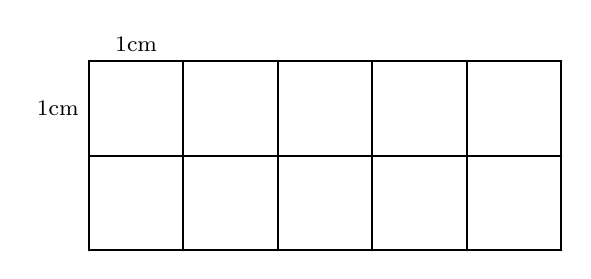
\begin{tikzpicture}[>=stealth,line join=round,line cap=round,font=\footnotesize,scale=0.6]
		\coordinate (A) at (0,0);
		\coordinate (B) at (2,0);
		\coordinate (C) at (4,0);
		\coordinate (D) at (6,0);
		\coordinate (E) at (8,0);
		\coordinate (F) at (10,0);
		\coordinate (A-1) at (0,-2);
		\coordinate (F-1) at (10,-2);
		\coordinate (A-2) at (0,-4);
		\coordinate (B-2) at (2,-4);
		\coordinate (C-2) at (4,-4);
		\coordinate (D-2) at (6,-4);
		\coordinate (E-2) at (8,-4);
		\coordinate (F-2) at (10,-4);
		\draw[line width=0.7pt,black] (A)--(F);
		\draw[line width=0.7pt,black] (A-1)--(F-1);
		\draw[line width=0.7pt,black] (A-2)--(F-2);
		\draw[line width=0.7pt,black] (A)--(A-2);
		\draw[line width=0.7pt,black] (B)--(B-2);
		\draw[line width=0.7pt,black] (C)--(C-2);
		\draw[line width=0.7pt,black] (D)--(D-2);
		\draw[line width=0.7pt,black] (E)--(E-2);
		\draw[line width=0.7pt,black] (F)--(F-2);
		\draw[line width=0.7pt,black] (A)--(B)node[above,pos=0.5]{1cm};
		\draw[line width=0.7pt,black] (A)--(A-1)node[left,pos=0.5]{1cm};
		\end{tikzpicture}
	\end{center}
	\choice
	{\True $14$}
	{$12$}
	{$10$}
	{$5$}
	\loigiai{
		Gọi $A$ là tập hợp hình vuông có cạnh $1$ cm.\\
		$B$ là tập hợp hình vuông có cạnh $2$ cm.\\
		$A$ và $B$ là hai tập hợp rời nhau.\\
		Số hình vuông trong hình là $n(A\cup B)=n(A)+n(B)=10+4=14$.}
\end{ex}
%%==========Câu 13
\begin{ex}%[Nguyễn Tấn Linh]%[1D2Y1-3]
	Trong mặt phẳng toạ độ $Oxy$, ở góc phần tư thứ nhất ta lấy $2$ điểm phân biệt; cứ thế ở các góc phần tư thứ hai, thứ ba, thứ tư lần lượt lấy $3,4,5$ điểm phân biệt (các điểm không nằm trên các trục toạ độ). Trong 14 điểm đó ta lấy $2$ điểm bất kỳ và nối chúng lại, hỏi có bao nhiêu đoạn thẳng cắt hai trục toạ độ, biết đoạn thẳng nối 2 điểm bất kì không qua $O$. 
	\choice
	{$91$}
	{$42$}
	{$29$}
	{\True $23$}
	\loigiai{
		\begin{center}
			\begin{tikzpicture}[>=stealth,line join=round,line cap=round,font=\footnotesize,scale=1]
			\draw[->] (-4,0)--(4,0)node[below]{$x$};
			\draw[->] (0,-4)--(0,4)node[right]{$y$};
			\fill (0,0)node[below left]{$O$}circle(1pt);
			\coordinate[label=above:$A$](A) at (2,3); 
			\coordinate[label=right:$B$](B) at (3,2);
			\coordinate[label=below left:$C$](C) at (-2,3.5);
			\coordinate[label=below left:$D$](D) at (-3,2.5);
			\coordinate[label=below left:$E$](E) at (-1,1);
			\coordinate[label=below left:$F$](F) at (-3,-1);
			\coordinate[label=below left:$G$](G) at (-2,-1.5);
			\coordinate[label=below left:$H$](H) at (-2.5,-2.5);
			\coordinate[label=below left:$I$](I) at (-3.5,-2);
			\coordinate[label=below left:$J$](J) at (2,-1);
			\coordinate[label=below left:$K$](K) at (3,-1.5);
			\coordinate[label=below left:$M$](M) at (1.5,-2);
			\coordinate[label=below left:$L$](L) at (2.5,-3);
			\coordinate[label=below left:$N$](N) at (1.5,-3.5);
			
			\fill[black](A)circle (1.5pt);
			\fill[black](B)circle (1.5pt);
			\fill[black](C)circle (1.5pt);
			\fill[black](D)circle (1.5pt);
			\fill[black](E)circle (1.5pt);
			\fill[black](F)circle (1.5pt);
			\fill[black](G)circle (1.5pt);
			\fill[black](H)circle (1.5pt);
			\fill[black](I)circle (1.5pt);
			\fill[black](J)circle (1.5pt);
			\fill[black](K)circle (1.5pt);
			\fill[black](L)circle (1.5pt);
			\fill[black](M)circle (1.5pt);
			\fill[black](N)circle (1.5pt);
			
			\draw[line width=0.7pt,black] (B)--(A)--(D)  (G)--(A)--(J);
			
			\end{tikzpicture}
		\end{center}
		Để chọn $2$ điểm trong $14$ điểm đã cho nối lại cắt hai trục toạ độ thì hai điểm đó phải thuộc hai góc phần tư đối đỉnh với nhau.\\
		TH1: Chọn 1 điểm ở góc phần tư thứ I và 1 điểm ở góc phần tư thứ III.\\
		Số đoạn thẳng tạo thành: $2.4=8$.\\
		TH2: Chọn 1 điểm ở góc phần tư thứ II và 1 điểm ở góc phần tư thứ IV.\\
		Số đoạn thẳng tạo thành: $3.5=15$.\\
		Theo quy tắc cộng ta có $8+15=23$ đoạn thẳng.}
\end{ex}
%%==========Câu 15

%%==========Câu 20
\begin{ex}%[Nguyễn Tấn Linh]%[1D2G1-3]
	Hỏi có tất cả bao nhiêu số tự nhiên chia hết cho $9$ mà mỗi số gồm $2011$ chữ số và trong đó có ít nhất hai chữ số $9$?
	\choice
	{$10^{2010}-16151\cdot 9^{2008}$}
	{$10^{2010}-16153\cdot 9^{2008}$}
	{$10^{2010}-16148\cdot 9^{2008}$}
	{\True $10^{2010}-16161\cdot 9^{2008}$}
	\loigiai{
		Đặt $A_1=\{0;9\}; A_2=\{1\}; A_3=\{2\}; A_4=\{3\};A_5=\{4\};A_6=\{5\};A_7=\{6\};A_8=\{7\}; A_9=\{8\}$.\\
		Gọi số cần tìm là $n=\overline{a_1a_2\ldots a_{2010}a_{2011}}\quad(a_1\neq 0)$.
		\begin{itemize}
			\item Xét các số tự nhiên chia hết cho 9, gồm 2011 chữ số
			\begin{itemize}
				\item Mỗi vị trí từ $a_2$ đến $a_{2011}$ đều có 10 cách chọn.
				\item $a_1$ phụ thuộc vào tổng $\left(a_2+a_3+\cdots +a_{2011}\right)$ nên có 1 cách chọn.
			\end{itemize}
			Vậy có $10^{2010}$ số.
			\item Xét các số tự nhiên chia hết cho 9, gồm 2011 chữ số nhưng không có mặt chữ số 9.
			\begin{itemize}
				\item $a_1$ có 8 cách chọn.
				\item Từ $a_2$ đến $a_{2010}$, mỗi vị trí đều có 9 cách chọn.
				\item $a_{2011}$ có 1 cách chọn.
			\end{itemize}
			Vậy có $8\cdot9^{2009}$ số.
			\item Xét các số tự nhiên chia hết cho 9, gồm 2011 chữ số trong đó có đúng 1 chữ số 9.
			\begin{itemize}
				\item Trường hợp $a_1=9$ ta có:
				\begin{itemize}
					\item Từ $a_2$ đến $a_{2010}$, mỗi vị trí đều có 9 cách chọn.
					\item $a_{2011}$ có 1 cách chọn.
				\end{itemize}
				Do đó có $9^{2009}$ số.
				\item Trường hợp $a_1\neq 9$ ta có:
				\begin{itemize}
					\item $a_1$ có 8 cách chọn.
					\item Có 2010 cách xếp chữ số 9.
					\item Ở 2008 vị trí còn lại, mỗi vị trí có 9 cách chọn.
					\item Vị trí cuối cùng có 1 cách chọn.
				\end{itemize}
				Do đó có $8.2010\cdot 9^{2008}$ số.
			\end{itemize}
		\end{itemize}
		Vậy số các số tự nhiên thỏa mãn yêu cầu bài toán là
		$$10^{2010}-\left(8\cdot 9^{2009}+9^{2009}+8\cdot2010\cdot9^{2008}\right)=10^{2010}-16161\cdot 9^{2008}\text{ số.}$$
	}
\end{ex}
\Closesolutionfile{ans}
%======================
\subsection{Bảng đáp án}
%\inputansbox{10}{ans/ANS-DANG-1}
